\chapter[A broadband radio study of PSR~J0250+5854]{A broadband radio study of PSR~J0250+5854: the slowest-spinning radio pulsar known}
\label{chapt: J0250}

Here I present simultaneous observations of the most slowly rotating known radio pulsar, PSR~J0250+5854, (period $P_1 = 23.5$~s) with FAST, two LOFAR international stations (UK608 at Chilbolton and DE601 at Effelsberg), and NenuFAR. The detections of this pulsar at 1250~MHz (FAST) and 57~MHz (NenuFAR) are the highest- and lowest-frequency published detections respectively to date, increasing the spectral coverage of this object by a factor of five. While PSR~J0250+5854 is slow, its continued radio emission beyond the canonical death line can be explained by, for example, the partially screened gap model. A flux density of $4\pm2$~$\upmu$Jy was measured at 1250~MHz giving an exceptionally steep spectral index of $-3.5^{+0.2}_{-1.5}$, with a turnover below $\sim95$~MHz. In conjunction with previous observations of this pulsar with the GBT and LOFAR Core, I show that the intrinsic profile width increases towards higher frequencies, contrary to the predictions of conventional radius-to-frequency mapping. This implies that the beam filling fraction is lower at low frequency. I use polarimetric data from FAST and LOFAR Core to constrain the emission geometry of PSR~J0250+5854, leading to the conclusion that its polar cap radio emission is produced at an absolute height of several hundreds of kilometres, similar to the other rotation-powered non-recycled pulsars, supporting the argument that emission height is relatively constant across the population. Finally, I draw a comparison between PSR~J0250+5854 and the other slow rotation-powered pulsars,  and contrast these with the radio-detected magnetars. I conclude that although they have similar spin periods, the magnetars have intrinsically wider radio beams than the slow rotation-powered pulsars. Consequently, the lower beaming fraction of the latter is what makes objects such as PSR~J0250+5854 so scarce. This work is under review for publication \citep{AWB+2021}.
% We present simultaneous observations of the most slowly-rotating known radio pulsar PSR~J0250+5854 (period $P=23.5$~s) with FAST, two LOFAR international stations (UK608 at Chilbolton and DE601 at Effelsberg), and NenuFAR. The detections with FAST at 1250~MHz and NenuFAR at 57~MHz are the highest- and lowest-frequency published detections respectively to date, and represent a five-fold increase in the spectral coverage of this object. We measure a flux density of $4\pm2$~$\upmu$Jy at 1250~MHz and an exceptionally steep spectral index of $-3.5^{+0.2}_{-1.5}$, with a turnover below $\sim$95~MHz. In conjunction with observations of this pulsar with the GBT and the LOFAR Core, I have shown that the intrinsic profile width increases towards higher frequencies, contrary to the predictions of conventional radius-to-frequency mapping. We used polarimetric data from FAST and the LOFAR Core to constrain the emission geometry of PSR~J0250+5854. This leads to the conclusion that its polar cap radio emission is produced at an absolute height of several hundreds of kilometres, similar to other rotation-powered pulsars and suggesting that it is relatively constant across the population. Finally, the results for PSR~J0250+5854, and those of other slowly-spinning rotation-powered pulsars are contrasted with those of the radio-detected magnetars. We conclude that magnetars have intrinsically wider radio beams than the slow rotation-powered pulsars, and that consequently the lower beaming fraction of the latter is what makes objects such as PSR~J0250+5854 so scarce.





\section{Introduction}
\label{sec: J0250 - introduction}

Pulsars are rapidly rotating, highly magnetised neutron stars; however, some pulsars rotate significantly less rapidly than others. In this chapter I discuss observations of PSR~J0250+5854, a radio pulsar with a period $P_1=23.5$~s discovered by \citet{TBC+2018} in the Low Frequency Array (LOFAR) Tied-Array All-Sky Survey \citep[LOTAAS;][]{SCB+2019}. It was detected with the LOFAR High Band Antenna array between 110--190~MHz, and with the Green Bank Telescope (GBT) between 300--400~MHz. It is the longest-period radio pulsar discovered to date, more than twice the period of the second slowest-spinning \citep[PSR~J2251$-$3711 at $P_1 = 12.1$~s;][]{MKE+2020} and almost three times slower than the well-studied 8.5~s pulsar PSR~J2144$-$3933 \citep{YMJx1999}. %Finding such a slow pulsar is rare, which may be explained by the fact that slower pulsars lose their ability to create electron-positron pairs and accelerate them sufficiently to produce the detectable coherent radio emission \citep{Sxxx1971}, and by their lower beaming fractions which make it less likely that they are visible to an Earthbound observer. In addition, there are practical issues with detecting slow pulsars due to selection effects making them significantly harder to identify in pulsar survey data if only a small number of pulses are present. The presence of red noise in periodicity searches further hinders their identification \citep[e.g.][]{LBH+2015,HKRx2017}.
Finding such a slow pulsar is rare, which may be explained by the fact that slower pulsars have lower beaming fractions which make it less likely that they are visible to an earthbound observer, and practical issues due to selection effects, making them significantly harder to identify in pulsar survey data (if only a small number of pulses are present). The presence of red noise in periodicity searches further hinders their identification \citep[e.g.][]{LBH+2015,HKRx2017}.


Furthermore, older, slower pulsars lose their ability to create electron-positron pairs and accelerate them sufficiently to produce the detectable coherent radio emission \citep{Sxxx1971}. Therefore, models for radio emission can be constrained by finding the slowest pulsars that are still active. As discussed in \citet{TBC+2018}, PSR~J0250+5854 occupies a relatively empty part of the $P$-$\dot{P}$ diagram, beyond the `death valley' as defined by \citet{CRxx1993} and the vacuum-gap curvature radiation death line proposed by \citet{ZHMx2000}, but it is consistent with the partially screened gap model \citep[e.g.][]{Sxxx2013}. Although PSR~J2144$-$3933 rotates almost three times faster, its much smaller spin-down rate $\dot{P} = 4.96\times10^{-16}$~s~s$^{-1}$ makes it more constraining for radio emission models \citep{MBMA2020}.


The extreme period of PSR~J0250+5854 places it in the company of the magnetars which have periods of 2--12~s \citep{OKxx2014}, but its spin-down rate of $\dot{P}~=~2.72\times10^{-14}$~s~s$^{-1}$ is around a thousand times smaller than those of the magnetars.  It also lies close to the parameter space inhabited by the population of X-ray Dim Isolated Neutron Stars (XDINSs). Of the seven brightest XDINSs, five have high magnetic dipole fields of the order of $10^{13}$--$10^{14}$~G which may mean they are related to magnetars \citep[][see Sec~\ref{sec: intro - general intro - pulsar population}]{Hxxx2007, KKxx2007}. These objects are detected only as soft thermal X-ray sources without radio counterparts. However, to date PSR~J0250+5854 remains undetected in X-rays, despite a dedicated \textit{Swift} X-Ray Telescope observation, which makes it difficult to confirm a connection between it and XDINS (see \citealt{TBC+2018} for details). Similarly, PSR~J0250+5854 has not shown any magnetar-like behaviour such as bursts, or any large radio variability as of yet.


This work details the first detection of PSR~J0250+5854 at frequencies between 1 and 1.5~GHz using the Five-hundred-metre Aperture Spherical radio Telescope (FAST), along with simultaneous observations with the UK608 and DE601 LOFAR international stations, and NenuFAR (New Extension in Nan\c{c}ay Upgrading loFAR). The NenuFAR detection at 57~MHz is the lowest-frequency detection of PSR~J0250+5854 published to date, and the FAST detection the highest, resulting in an extension by a factor of $\sim$5 in spectral coverage of this unique source in the radio domain. Upon its discovery \citet{TBC+2018} were able to detect PSR~J0250+5854 over the frequency range between 120 and 350~MHz, and fitted a spectral index of $-2.6\pm0.5$. However, with no detection of the pulsar at around 1500~MHz using the Lovell and Nan\c{c}ay radio telescopes, nor a detection with the core LOFAR Low Band Antenna stations (at 55~MHz), uncertainty remained over the broadband shape of the radio spectrum. 


A key part of understanding the pulsar emission mechanism lies in studying their radio frequency evolution. This is particularly relevant for pulsars such as PSR~J0250+5854 which are on the cusp of the death line. Multi-wavelength observations can provide information on features including the spectral index (how the flux of the pulsar changes with frequency), and changes in the shape and polarisation properties of the radio beam.

Measurements of pulsar radio spectra from a large population began with \citet{Sxxx1973}, \citet{MMxx1980} and \citet{IKMS1981} using frequencies around and below 100~MHz. Most pulsars were found to have steep spectra which could be modelled with a simple power law $S_\nu \propto \nu^k$, where $S_\nu$ is the mean flux density at some frequency $\nu$ and $k$ is the spectral index. For some pulsars deviations from this relation were identified in the form of a turn-over at low frequencies which can be attributed to absorption mechanisms, whilst others show a cut-off at high frequencies due to a steepening or break in the spectrum \citep{Sxxx1973}. Two recent studies of radio pulsar spectral indices have been performed by \citet{BKK+2016} and \citet{JSK+2018}. \citet{BKK+2016} studied the spectra of 165 non-recycled pulsars in the Northern sky with LOFAR, and found that 124 were best fitted by the simple power-law model, whilst the remaining 41 were fitted with a broken power law. They found a mean spectral index of $k = -1.4$. Similarly, \citet{JSK+2018} studied 441 pulsars and found that 79~per~cent obeyed a simple power-law relation. The spread of spectral indices is described by a shifted log-normal distribution with a weighted mean of $-1.60\pm0.03$ and a standard deviation of 0.54, and this study covered centre frequencies of 728, 1382, and 3100~MHz using the Parkes radio telescope.

With its period of 23.5~s, PSR~J0250+5854 has an extremely large light-cylinder (with a radius $R_\mathrm{LC} = cP_1/2\pi =  1.123\times10^{6}$~km, where $c$ is the speed of light), and hence a tiny polar cap which connects to the open-field-line region (see Sec.~\ref{sec: intro - general intro}). The diameter of the polar cap is $D_\mathrm{PC} \approx 2R\sqrt{R/R_\mathrm{LC}} \approx~60$~m, where $R = 10$~km is the canonical neutron star radius \citep[e.g.][]{Sxxx1971}. By comparison, a pulsar with a period $P_1 = 0.5$~s would have $D_\mathrm{PC} \approx 410$~m. This implies that for typical emission heights of hundreds of kilometres, the radio beam of PSR~J0250+5854, and hence the duty cycle of its radio pulse, can be expected to be very narrow. Indeed \citet{TBC+2018} reported a pulse width of only $\sim$1$\degr$ at 129, 168, and 350~MHz. 

The shapes of pulse profiles after correcting for propagation effects (see Sec.~\ref{sec: intro - observation processing - ISM effects}) are in general observed to be frequency-dependent. Often, the profile width is seen to decrease with increasing frequency, which suggests that higher-frequency emission is produced lower in the magnetosphere. This correlation is known as radius-to-frequency mapping (RFM hereafter), and was first theorised by \citet{RSxx1975} who related the emission height to the local plasma frequency in the magnetosphere. The electron density (and hence plasma frequency) is expected to decrease with increasing altitude ($\rho \propto r^{-3}$), thereby predicting that the radio beam expands with decreasing frequency. However, a number of pulsars have been found to deviate from this relation \citep[e.g.][]{Txxx1991, CWxx2014,PHS+2016} -- this suggests the same set of magnetic field lines are not necessarily active at all frequencies (or emission heights), resulting in the appearance and disappearance of profile components with observing frequency \citep[e.g.][]{Cxxx1978, MRxx2002}. This can obfuscate the geometrical interpretation of measured profile widths, and is discussed further in Sec.~\ref{sec: J0250 - discussion - profile width}. Radio polarisation data can help in disentangling these effects, which is further explored for PSR~J0250+5854 in Sec.~\ref{sec: J0250 - analysis - polarisation and geometry}, although degeneracies often remain \citep[e.g.][]{KJW+2010}.

The structure of this chapter is as follows. In Sec.~\ref{sec: J0250 - observations} the new observations are described, followed by a brief explanation of the radio-frequency interference (RFI) excision techniques used. The analysis of the data described in Sec.~\ref{sec: J0250 - analysis} is divided into three parts: pulse profile evolution with frequency, polarisation properties, and the spectral shape of the pulsar flux density. These results are then discussed in a broader context in Sec.\ref{sec: J0250 - discussion}, and the conclusions are summarised in Sec.~\ref{sec: J0250 - conclusions}.




















\section{Observations}
\label{sec: J0250 - observations}

As part of a shared-risk proposal, PSR~J0250+5854 was observed on 22 May 2019 with FAST, a facility built and operated by the National Astronomical Observatories, Chinese Academy of Sciences \citep{NLJ+2011,LWQ+2018}. The central beam of the 19-beam receiver operating between 1 and 1.5~GHz \citep{JTH+2020} was used. At the time of these observations FAST was commissioned, and full polarisation information is available -- the issues detailed in Chapters~\ref{chapt: J1926} and \ref{chapt: J1518} have now been resolved. Two LOFAR international stations -- UK608 (United Kingdom) and DE601 (Germany) --- and NenuFAR (France) provided overlapping observations. Chilbolton is home to the UK LOFAR station UK608, formally known as the Rawlings Array, and the DE601 station is located at Effelsberg\footnote{DE601 was operated as part of the German Long Wavelength (GLOW) consortium at the time of these observations, in a coherently dedispersed folding mode.}. They each consist of two sub-arrays: the High Band Antenna (HBA; 110--240~MHz) and Low Band Antenna (LBA; 10--90~MHz) \citep{HWG+2013,SHA+2011}, although only the HBA were used in this project and the bandwidth was limited to 110--190~MHz. At the time of these observations, NenuFAR consisted of 52 groups of 19 dual-polarised antennas, operating between 10 and 85~MHz \citep{ZDT+2020}. It is located alongside and extends the capabilities of the Nan\c{c}ay LOFAR station (FR606). Table \ref{tab: J0250 - observations} gives a summary of the overlapping observations conducted. The LOFAR international stations observed PSR~J0250+5854 over the full duration of the FAST observations, and in the case of NenuFAR significantly longer.

Prior to observing PSR~J0250+5854, FAST performed a $\sim$15-minute observation of a well-known, bright pulsar PSR~J0139+5814 to validate the set-up of the observing system. A noise diode signal was injected into the FAST multibeam receiver to facilitate polarisation calibration (see Sec.~\ref{sec: intro - observation processing - polarisation calibration}). PSR~J0250+5854 was observed for two consecutive hours, interspersed with noise diode observations. Finally, the BL Lacertae object J0303+472 \citep{VVxx2006} was observed for purposes of flux calibration (see Sec.~\ref{sec: intro - observation processing - flux calibration}) -- this source was chosen due to its proximity to PSR~J0250+5854.

All data were folded and de-dispersed with \textsc{dspsr} \citep{SBxx2011} using the ephemeris and dispersion measure (DM) reported in \citet{TBC+2018} to form a pulse sequence. De-dispersion was done coherently for the DE601, UK608, and NenuFAR data, and incoherently for the FAST data. Flux and polarisation calibration were done using the \texttt{pac} program in \textsc{psrchive} \citep{SMJR2010}. Further processing made use of \textsc{psrsalsa} \citep{Wxxx2016} and is described later in this chapter.

Although not part of the simultaneous observations, this project also made use of an observation of PSR~J0250+5854 using the LOFAR Core stations \citep{HWG+2013} conducted on 28 October 2017. This was part of a run of observations conducted by \citet{TBC+2018}, but is a different data set to the profiles shown in that paper. This LOFAR Core observation was similarly processed with \textsc{psrchive}.

\begin{landscape} % Maybe not landscape, but needs tweaking!
    \begin{table}
        \centering
        \caption[Summary of the simultaneous observations of PSR~J0250+5854]{Observation properties of the analysed observations. There is a full overlap of the data for the period during which FAST was recording data for PSR~J0250+5854 on 22 May 2019 (these observations are denoted with a *). `Resolution' is the number of samples (pulse longitude `bins') per pulse period. The GBT and LOFAR Core observations were performed earlier, on 2017-10-25 and 2017-10-28 respectively.}
        \label{tab: J0250 - observations}
        \begin{tabular}{crrrrrrrc} % 6 columns, alignment for each
            \hline
            Observation & Centre freq. & Bandwidth & No. freq. & Start time & No. pulses & Length & Resolution & Full Stokes\\
            & (MHz) & (MHz) & channels & (UTC) & & (hh:mm:ss) & (No. Bins)&\\
            \hline
            FAST *        & $1250.00$ & $500.0$   & 4096 & 02:34:07  & 100   & 00:39:13  & 8192 & Y\\
            FAST *	    & $1250.00$ & $500.0$   & 4096 & 03:31:23 & 153   & 01:00:01  & 8192 & Y\\
            DE601 *        & $158.55$  & $71.4$    & 488  & 01:56:19  & 417   & 02:43:34  & 1024  & N \\
            UK608 *  & $149.71$  & $95.2$    & 1952 & 02:02:50  & 382   & 02:29:50  & 8192  & N\\
            NenuFAR *     & $56.54$   & $75.0$    & 384  & 02:03:18  & 1528  & 09:59:21  & 2048  & N \\
            \hline
            GBT & 350.00 & 100.0 & 4096 & 11:54:28 & 242 & 01:34:55 & 8192 & N\\
            LOFAR Core & 148.93 & 78.1 & 400 & 23:57:16 & 152 & 00:59:49 & 16384 & Y\\
            \hline
        \end{tabular}
    \end{table}
    \end{landscape}











\subsection{Data cleaning techniques}
\label{sec: J0250 - observations - cleaning}

PSR~J0250+5854 has a low flux density which, in combination with its extraordinarily long period, makes the analysis highly susceptible to radio-frequency interference (RFI) that affects the baseline level during a rotation period. A somewhat different approach to mitigate the effects of RFI was taken for the different datasets, guided by the nature of the RFI present.

In all datasets the worst-affected frequency channels were identified and excluded from further analysis. The FAST data were affected by stochastic baseline variations that persisted throughout the observation, with a scale somewhat larger than the pulsar's duty cycle. These baseline variations were removed using the \texttt{pmod} program in \textsc{psrsalsa} by subtracting sinusoids plus a constant offset fitted to the off-pulse region for each rotation of the star in each frequency channel and Stokes parameter independently. This ensures that the mean intensity of the emission in the off-pulse region is zero. The sinusoids were harmonics of the pulse period, and were fitted up to the 23\textsuperscript{rd} harmonic. These sinusoids have periods which significantly exceed the duty cycle of the pulsar to ensure that the shapes of the pulses would not be affected by this process.

The character of the RFI in the DE601 and UK608 observations was very different, appearing as short, bright, impulsive spikes orders of magnitude brighter than the pulsar signal. An effective approach to mitigation was to iteratively clip the brightest samples for each rotation of the star and each frequency channel individually. Again, this made use of \textsc{psrsalsa}. The clipping was done conservatively to ensure that the pulsar signal remained unaffected. With the worst RFI suppressed, the remaining RFI and baseline variations were reduced using the same method described for the FAST data.

The NenuFAR data were recorded during the commissioning phase of the instrument with a coherent de-dispersion pipeline \citep[LUPPI;][]{BGT+2020} operating in single-pulse mode. The observations were folded with \textsc{dspsr} and a polynomial of degree two was subtracted from the baseline of each sub-integration to suppress the effect of bandpass variations. The data from two frequency bands were appended after correcting for the appropriate delay\footnote{The observation was recorded in two sub-bands which have a slight phase offset when de-dispersed, and so had be aligned manually. This is only necessary for older NenuFAR observations conducted before the `early science' phase.}. The frequency-resolved observation was cleaned using a modified version of \textsc{coastguard} \citep{LKG+2016} and final processing was done with \textsc{psrsalsa} in the same way as with the FAST data.



\section{Analysis and results}
\label{sec: J0250 - analysis}

\subsection{Profile morphology and width evolution}
\label{sec: J0250 - analysis - profile widths}

Figure \ref{fig: J0250 - profiles} shows the integrated pulse profile of PSR~J0250+5854 as observed simultaneously by the four telescopes, in order of descending frequency. The profile observed by the GBT at 350~MHz from \citet{TBC+2018} is also included, as is a LOFAR Core detection at 149~MHz (an observation from 28 October 2017). The profiles for the LOFAR international stations and NenuFAR are obtained from the full-length observation rather than only the overlap period with the FAST observation to increase the signal-to-noise ratio. This is motivated by the fact that there is no evidence that the profile shapes were changing during these observations. This also implies that although a relatively low number of pulses ($<1000$) were observed, meaning that the average pulse profiles cannot be expected to be fully stable because of pulse-to-pulse variability \citep[e.g.][]{HMTx1975,RRxx1995,LKL+2012}, this is not a significant issue for this data analysis.

\begin{figure}
    \begin{center}
    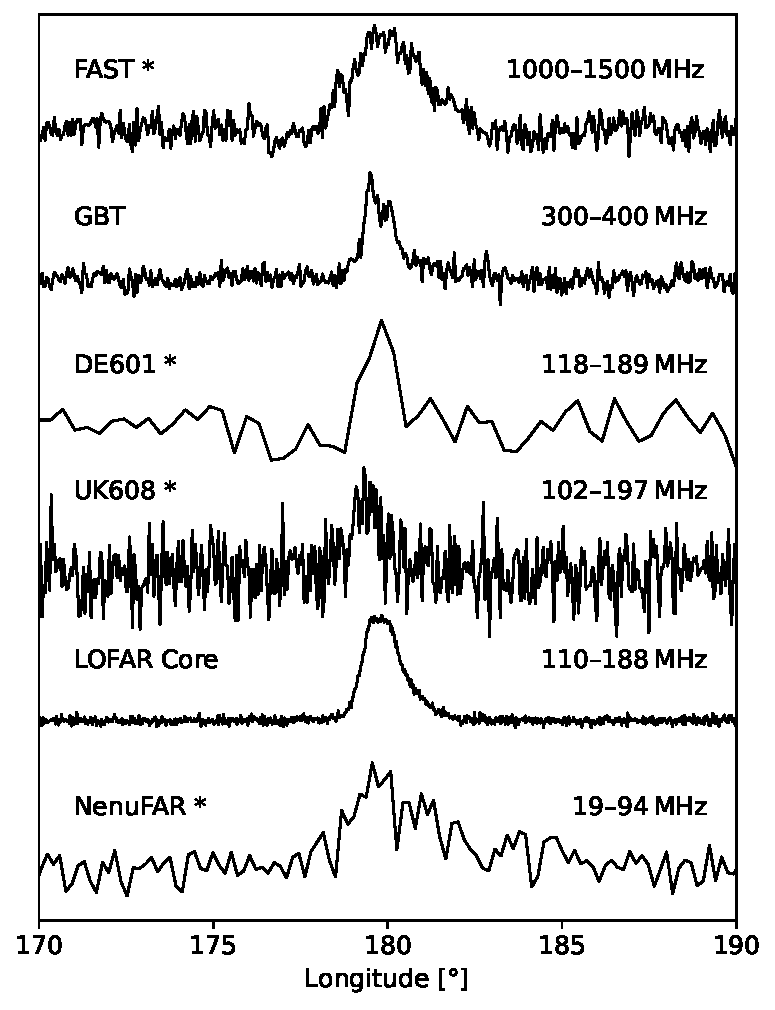
\includegraphics[width=0.75\textwidth]{Figures/J0250/profiles.pdf}
    \caption[Multi-frequency profiles of PSR~J0250+5854]{ The pulse profiles of PSR~J0250+5854 at different radio frequencies. The top profile is from FAST (1250~MHz), followed by GBT (350~MHz), then DE601 (154~MHz), UK608 (150~MHz), LOFAR Core (149~MHz), and finally NenuFAR (57~MHz). The FAST, DE601, and UK608 observations are overlapping in time, and are aligned using the known DM and after accounting for geometric delays. The FAST profile is derived from the combination of the two observations. The profiles from the non-simultaneous observations and NenuFAR were visually aligned. The simultaneous observations are denoted with an asterisk (*).}
    \label{fig: J0250 - profiles}
    \end{center}
\end{figure}

The profiles of the simultaneous observations in Fig.~\ref{fig: J0250 - profiles} were aligned by correcting for geometric delays associated with the difference in location of the telescopes (taking the right ascension of PSR~J0250+5854 to be $02^\mathrm{h}50^\mathrm{m}17\fs78$ and the declination to be $+58\degr54'01\farcs3$, as measured by \citealt{TBC+2018}). In addition, the dispersive delay associated with the propagation of the signal through the interstellar medium (ISM) was accounted for by using a DM of $45.281\pm0.003\ \mathrm{cm}^{-3}\ \mathrm{pc}$ \citep{TBC+2018}. There is no evidence for a change in the DM as the value derived from this NenuFAR data is $45\pm1\ \mathrm{cm}^{-3}\ \mathrm{pc}$, hence consistent with the DM used. The long period of PSR~J0250+5854 means the uncertainty on the DM translates to an uncertainty on the dispersion delay between the highest frequency (FAST; 1250 MHz) and lowest frequency (NenuFAR; 57 MHz) observations of 3.9~ms, or around one pulse longitude bin at the highest resolution shown in Fig.~\ref{fig: J0250 - profiles} (for the FAST and UK608 data) so is of little concern for this long-period pulsar. The NenuFAR data were obtained during commissioning phase of that telescope and so could not be aligned in this way; the peak of this profile was therefore aligned visually with the UK608 profile peak.

Only the GBT profile has a clear double-peaked profile morphology. Although single-peaked, the LOFAR Core profile, with a flat profile peak, and the somewhat asymmetric FAST profile can be taken as evidence for a more complicated profile structure. Inspecting the profiles in Fig.~\ref{fig: J0250 - profiles}, it is evident that the profile width at frequencies below that of the FAST observation are significantly narrower, opposite to the expected behaviour by RFM. 

The NenuFAR profile, corresponding to the lowest frequency, is broader still and distinctly skewed. Given the steep rise followed by an exponentially decreasing tail, this can be attributed to scattering of the emission in the ISM (see Sec.~\ref{sec: intro - observation processing - ISM effects - scattering}). This is a strongly frequency-dependent effect with a power-law relationship between the scattering timescale and frequency, with a power law index of around $-4$ \citep{SDOx1980,PulsarAstronomy, GKK+2017}. This indicates that the scattering timescale for the NenuFAR data is around 50 times greater than at the UK608 centre frequency, which explains why only the NenuFAR profile is significantly affected. The NenuFAR profile is consistent with an intrinsic profile width which is equal to that observed at $\sim$150~MHz, albeit broadened by scattering. This is demonstrated in Fig.~\ref{fig: J0250 - nenufar scattering} where the NenuFAR profile is compared with a von Mises function with a width equal to that of the UK608 profile, and convolved with an exponential scattering tail with an e-fold timescale of 0.1~s. This timescale is consistent with the observed relationship between the DM and scattering timescale \citep[e.g.][]{BCC+2004,IJWx2019}. Therefore, scattering can fully explain the observed frequency evolution of the profile between 60 and 150~MHz, although given that its low signal-to-noise ratio (S/N) makes it nearly impossible to resolve the profile reliably across the frequency band, the possibility of intrinsic profile evolution can not be fully excluded. On the other hand, the LOFAR Core profile with a high S/N also shows a somewhat elongated tail. No evolution of this tail is observed across the bandwidth of the observation, excluding scatter broadening being the main cause for the tail observed in that frequency range -- this instead appears to be an intrinsic feature of the profile. Whilst the observation covers a very similar frequency range, the S/N is too low in the UK608 profile to expect this tail to stand out. So the conclusion is that only the NenuFAR profile shows clear evidence for being scatter-broadened.
\begin{figure}
    \begin{center}
        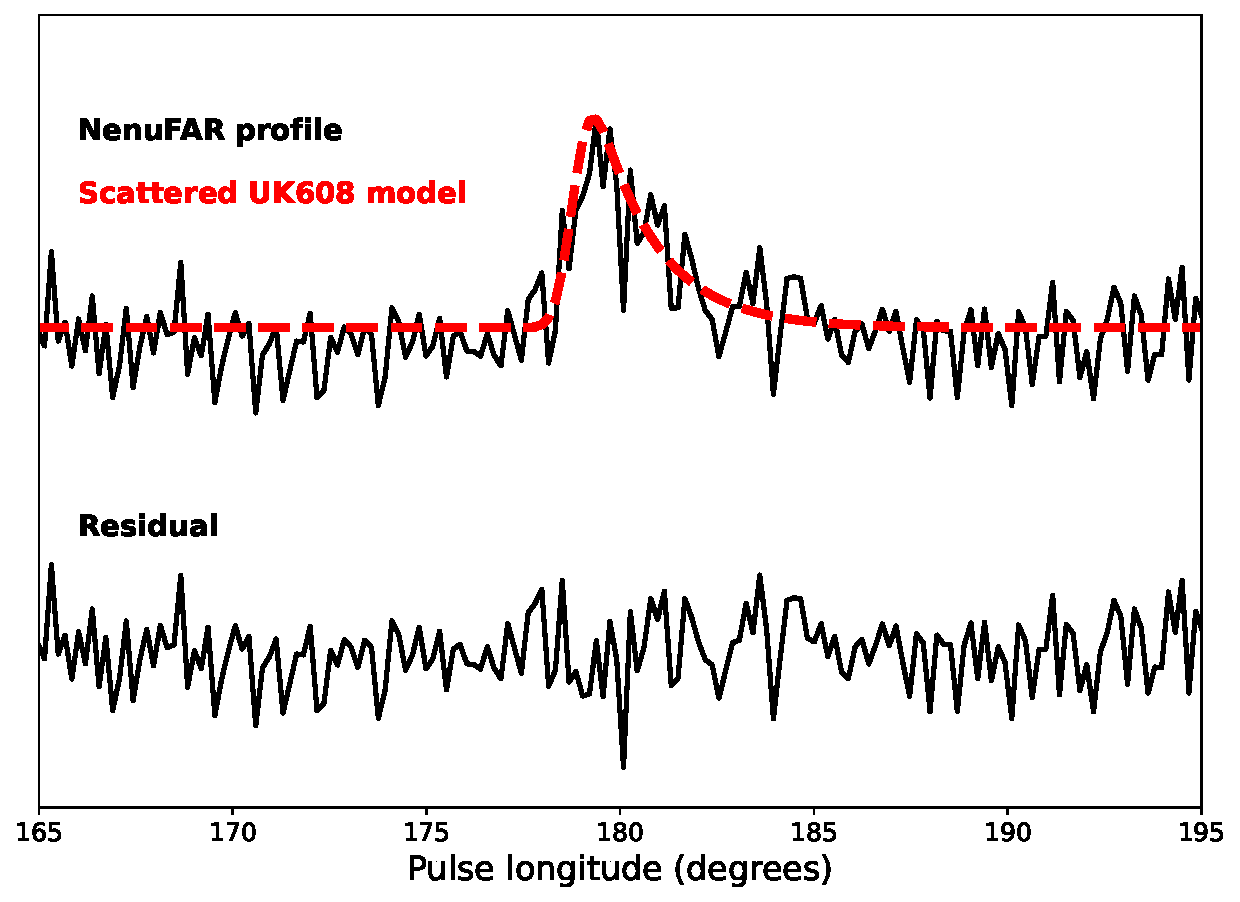
\includegraphics[width=0.7\textwidth]{Figures/J0250/nenufar_scattering.pdf}
        \caption[Evidence for scattering in the NenuFAR profile of PSR~J0250+5854]{The NenuFAR profile (top) compared to a smoothed UK608 profile that has been convolved with a scattering tail (red dashed curve). No significant signal remains in the residuals (bottom).}
        \label{fig: J0250 - nenufar scattering}
    \end{center}
\end{figure}

To confirm and quantify the pulse broadening at higher frequencies, the profile widths as shown in Fig.~\ref{fig: J0250 - profiles} were measured by fitting von Mises functions to each profile using \textsc{psrsalsa}. This smooth mathematical description of the profile allows the width to be measured objectively, without being strongly affected by (white) noise. Two components were used to model the higher S/N profiles (LOFAR Core, GBT) but including more than one component for weaker profiles would result in over-fitting. The uncertainty on each measurement was calculated using bootstrapping, where for each iteration a pulse phase-rotated version of the baseline was added to the profile. This ensures that both the statistical error arising from the presence of white noise as well as residual baseline variations are accounted for. The estimated full width at half maximum ($W_{50}$) of the profiles in Fig.~\ref{fig: J0250 - profiles} are presented in Tab.~\ref{tab: J0250 - W50}.
\begin{table}
    \centering
    \caption[The measured profile widths of PSR~J0250+5854 across the observed frequency range]{The profile width at half maximum ($W_{50}$) of PSR~J0250+5854 as a function of frequency, measured by fitting von Mises functions to each profile shown in Fig.~\ref{fig: J0250 - profiles}. These measurements are taken from the profiles as observed, and so includes the effect of scatter broadening in the case of the NenuFAR profile.}
    \label{tab: J0250 - W50}
    \begin{tabular}{lcc}
        \hline
        Telescope & Centre freq. (MHz) & $W_{50}~(\degr)$ \\
        \hline
        FAST & 1250 & $2.4\pm0.1$ \\
        GBT & 350 & $1.08\pm0.07$ \\
        DE601 & 154 & $0.9\pm0.1$ \\
        UK608 & 150 & $0.9\pm0.1$ \\
        LOFAR Core & 149 & $1.21\pm0.03$ \\
        NenuFAR & 57 & $2.8\pm0.4$ \\ 
    \end{tabular}
\end{table}
To further investigate the frequency evolution of the profile width, the widths were also determined after dividing the FAST data into four frequency sub-bands. Figure~\ref{fig: J0250 - width evolution} shows the profile width against frequency for the profiles shown in Fig.~\ref{fig: J0250 - profiles} (black) and the FAST sub-bands (blue).

\begin{figure}
    \begin{center}
        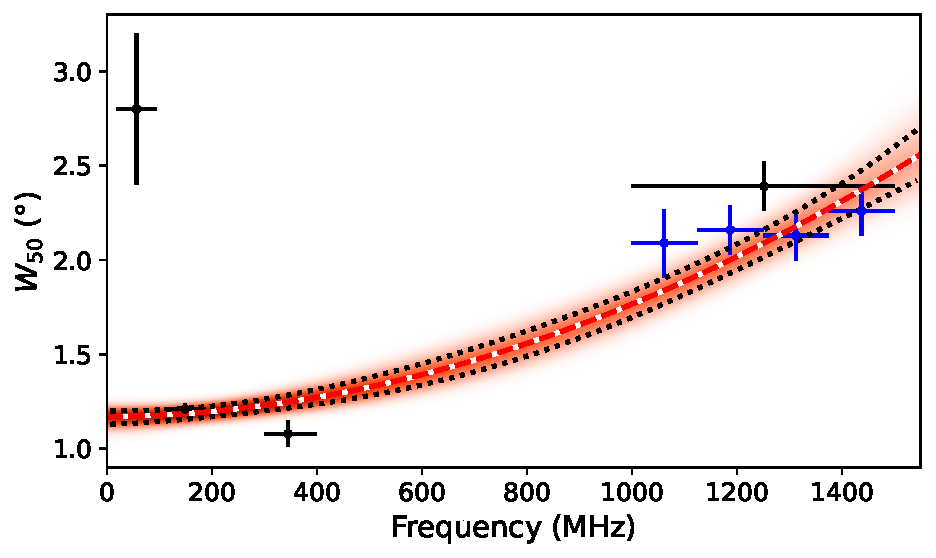
\includegraphics[width=0.75\textwidth]{Figures/J0250/thorsett_relation.pdf}
        \caption[Broadening of the profile with increasing frequency]{Evolution of the profile width of PSR~J0250+5854 with observing frequency. Points in black correspond to the profiles shown in Fig.~\ref{fig: J0250 - profiles} and blue points are the profile widths of the four FAST sub-bands. The red and white dashed line represents the model of frequency evolution in Eq.~\eqref{eq: J0250 - thorsett relation} which was fitted to the FAST sub-bands, GBT, UK608, and LOFAR Core data (NenuFAR was excluded because it is affected by scattering). A distribution of fits was calculated using bootstrapping techniques, and is represented by the red colour gradient. The black dotted lines indicate the 68~per~cent confidence interval of this distribution. The horizontal error bars indicate the bandwidth of a given observation.}
        \label{fig: J0250 - width evolution}
    \end{center}
\end{figure}

The evolution of profile width with frequency $\nu$ was modelled using the relation
\begin{equation}
\label{eq: J0250 - thorsett relation}
    W_{50} = A\nu^B + C,
\end{equation}
where $A$, $B$, and $C$ are constants \citep{Txxx1991, CWxx2014}. The function in Eq.~\eqref{eq: J0250 - thorsett relation} was fitted to the profile widths measured from the LOFAR Core, UK608, GBT, and FAST sub-band data. The NenuFAR profile was omitted to avoid scattering by the ISM affecting the results, and the DE601 and UK608 data were omitted because of their low S/N compared to the LOFAR Core data at a similar frequency. The horizontal error bars represent the bandwidth of a given observation. During fitting of Eq.~\eqref{eq: J0250 - thorsett relation} the frequency of each observation was allowed to vary uniformly within these limits to account for the frequency-dependence of the profile width within the observed band. The distribution of fitted trend lines is shown in the red gradient plot in Fig.~\ref{fig: J0250 - width evolution}. The black dotted lines bound the 68~per~cent confidence interval of the distribution, as a function of frequency. The red and white dashed line represents the optimal fit to the data, and the power-law exponent of Eq.~\eqref{eq: J0250 - thorsett relation} is $B = 1.9 \pm 0.4$. These findings are discussed further in Sec.~\ref{sec: J0250 - discussion}.







\subsection{Polarisation and geometry}
\label{sec: J0250 - analysis - polarisation and geometry}

Polarisation calibration was performed on the FAST data using \textsc{psrchive}, making use of a pulsed noise diode signal injected into the 19-beam receiver. The multibeam receiver maintains a fixed orientation with respect to the sky during the observation by rotating within the focus cabin, so no parallactic angle corrections are required. After calibration, the polarised pulse profile of PSR~J0139+5814 (not shown, see also Sec.~\ref{sec: J0250 - observations}) is in excellent agreement with the results of \citet[publicly available on the European Pulsar Network (EPN) database\footnote{\url{http://www.epta.eu.org/epndb/}}]{GLxx1998}, confirming that the polarisation data from FAST is now reliable. The LOFAR Core data were not polarisation-calibrated using the LOFAR station beam model, but rather tied-array addition which incorporates data from different tiles and stations using the station calibration tables to account for the delays between them \citep[more detail can be found in ][]{SBG+2019}. The signs of Stokes $V$ and the position angle curve had to be flipped in order to agree with convention \citep[e.g.][see also Sec.~\ref{sec: intro - emission models - polarisation - conventions}]{EWxx2001}, a correction that was also applied to the FAST data. The Faraday rotation measure towards PSR~J0250+5854, $\mathrm{RM}=-54.65\pm0.02$~rad~m$^{-2}$, was measured by applying RM synthesis \citep{BBxx2005} to the LOFAR Core polarisation data. This is consistent with the RM measured using the FAST data, although this has a larger uncertainty due to the higher observing frequency. Therefore, the linear polarisation data for both observations were de-Faraday-rotated using the LOFAR value.

\begin{figure}
    \begin{center}
        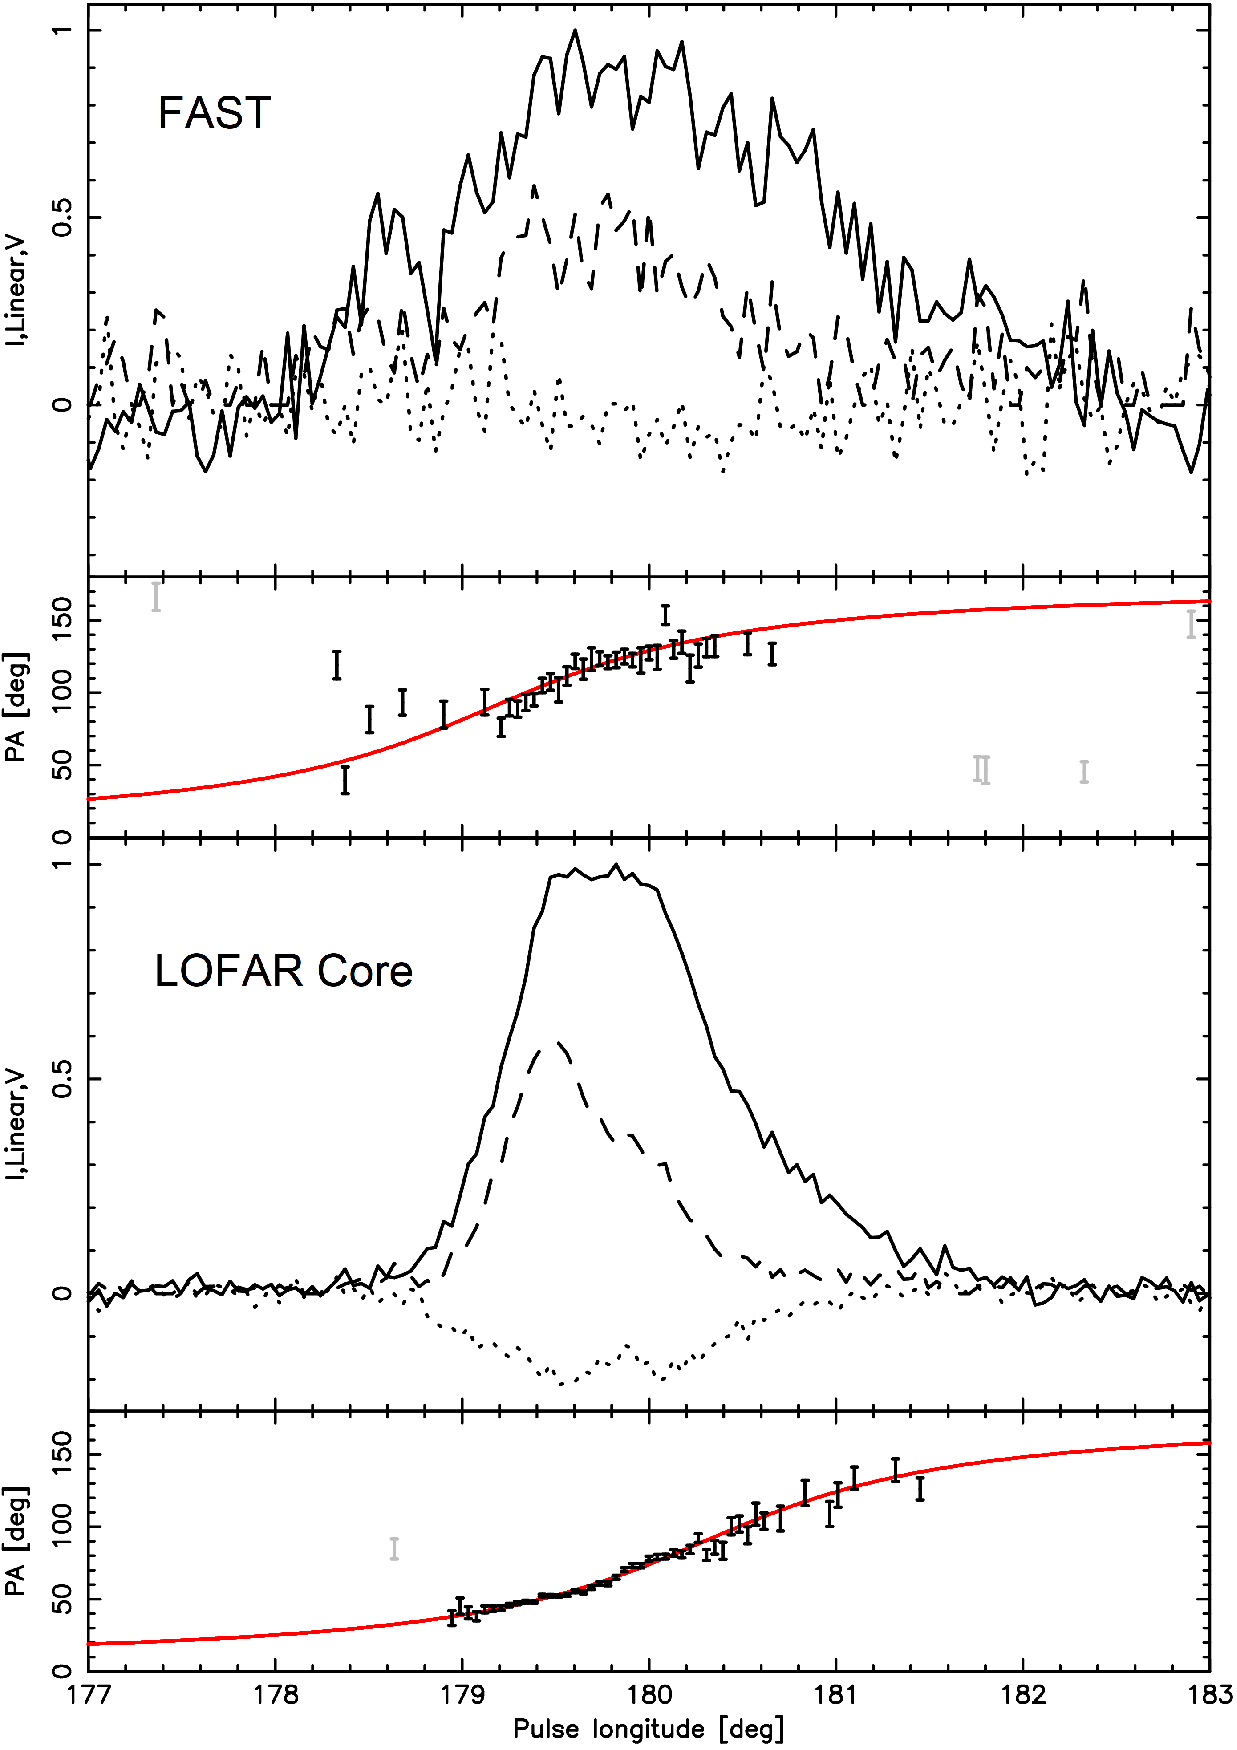
\includegraphics[width=0.75\textwidth]{Figures/J0250/polarised_profiles.pdf}
        \caption[The polarised FAST and LOFAR Core profiles of PSR~J0250+5854]{The polarised profile of PSR~J0250+5854, observed with FAST (upper plot) and LOFAR Core (lower plot). Total intensity is shown as the solid line, and linear and circular polarisation as dashed and dotted respectively. The lower panel of each plot shows the variation of position angle of linear polarisation with pulse longitude. The RVM (red curve in the online version) was fitted to the LOFAR Core data, and the same curve (with appropriate horizontal and vertical offset applied; see text) is shown for the FAST data. The darker PA points were those used in the fitting.}
        \label{fig: J0250 - polarised profiles}
    \end{center}
\end{figure}
   
In Figure~\ref{fig: J0250 - polarised profiles} the polarised profile of PSR~J0250+5854 is shown as observed with FAST (first panel), and the LOFAR Core data (third panel). In both, the solid line is total intensity. The pulse profile has a moderate degree of linear polarisation (dashed), which was de-biased according to \citet{WKxx1974}. There is negative circular polarisation (dotted line) in the LOFAR observation, and a hint of the same in the FAST data. The position angle (PA, $\psi$) as a function of pulse longitude is shown in the second and fourth panels of Fig.~\ref{fig: J0250 - polarised profiles}, which relates to the Stokes $Q,\ U$ parameters via $\psi = 0.5 \arctan(U/Q)$. Its functional shape can be explained by the Rotating Vector Model \citep[RVM;][]{RCxx1969}, a geometric model which links the observed changes in PA with pulse longitude $(\phi)$ to the orientation of the magnetic field lines with respect to the observer (see Sec.~\ref{sec: intro - emission models - polarisation - RVM}).

To fit the RVM (Eq.~\eqref{eq: intro - RVM}), a grid search was conducted over the inclination angle of the magnetic axis, $\alpha$, and the impact parameter of the observer's line of sight with respect to the magnetic axis, $\beta$, as was done for PSR~J1926$-$0652 in Chapter~\ref{chapt: J1926}. This was performed for the LOFAR Core observation and the best fit to the observed PA points is shown in Fig.~\ref{fig: J0250 - polarised profiles} (only the darker PA points were fitted). The same curve is used for both the LOFAR and FAST data after applying an offset in PA to account for the fact that no absolute PA calibration has been performed, and allowing for a shift of the inflection point in longitude. As will be discussed in Sec.~\ref{sec: J0250 - discussion}, the offset of $1.2\pm0.2\degr$ in the PA inflection point between the FAST and LOFAR Core data is suggestive of emission at different radio frequencies originating at different heights in the magnetosphere. However, the functional shapes of the LOFAR and FAST PA data are identical within the errors, as expected when a dipolar field line configuration determines the shape -- the reduced-$\chi^2$ of the RVM fit to the LOFAR Core data is 1.74 (52 degrees of freedom), and the reduced-$\chi^2$ of the same curve fitted to the FAST data was 1.45 (31 degrees of freedom). We therefore will only consider the RVM fit to the higher S/N LOFAR Core data. 

The goodness-of-fit of the RVM to the observed $\psi$ as a function of $\phi$ is parametrised by the reduced-$\chi^2$ and its variation is shown in Fig.~\ref{fig: J0250 - banana} for the LOFAR Core data (see \citealt{RWJx2015a} for details of the methodology used). The darker shading corresponds to lower reduced-$\chi^2$ values and so a better fit. The black contours indicate $1\sigma$, $2\sigma$ and $3\sigma$ confidence intervals. As can be expected for a pulsar with a very small duty-cycle, $\alpha$ and $\beta$ are highly correlated. The fit confirms that $\beta$ must be small ($<1.8\degr$), however the magnetic inclination $\alpha$ is unconstrained from RVM fitting alone.
\begin{figure}
    \begin{center}
        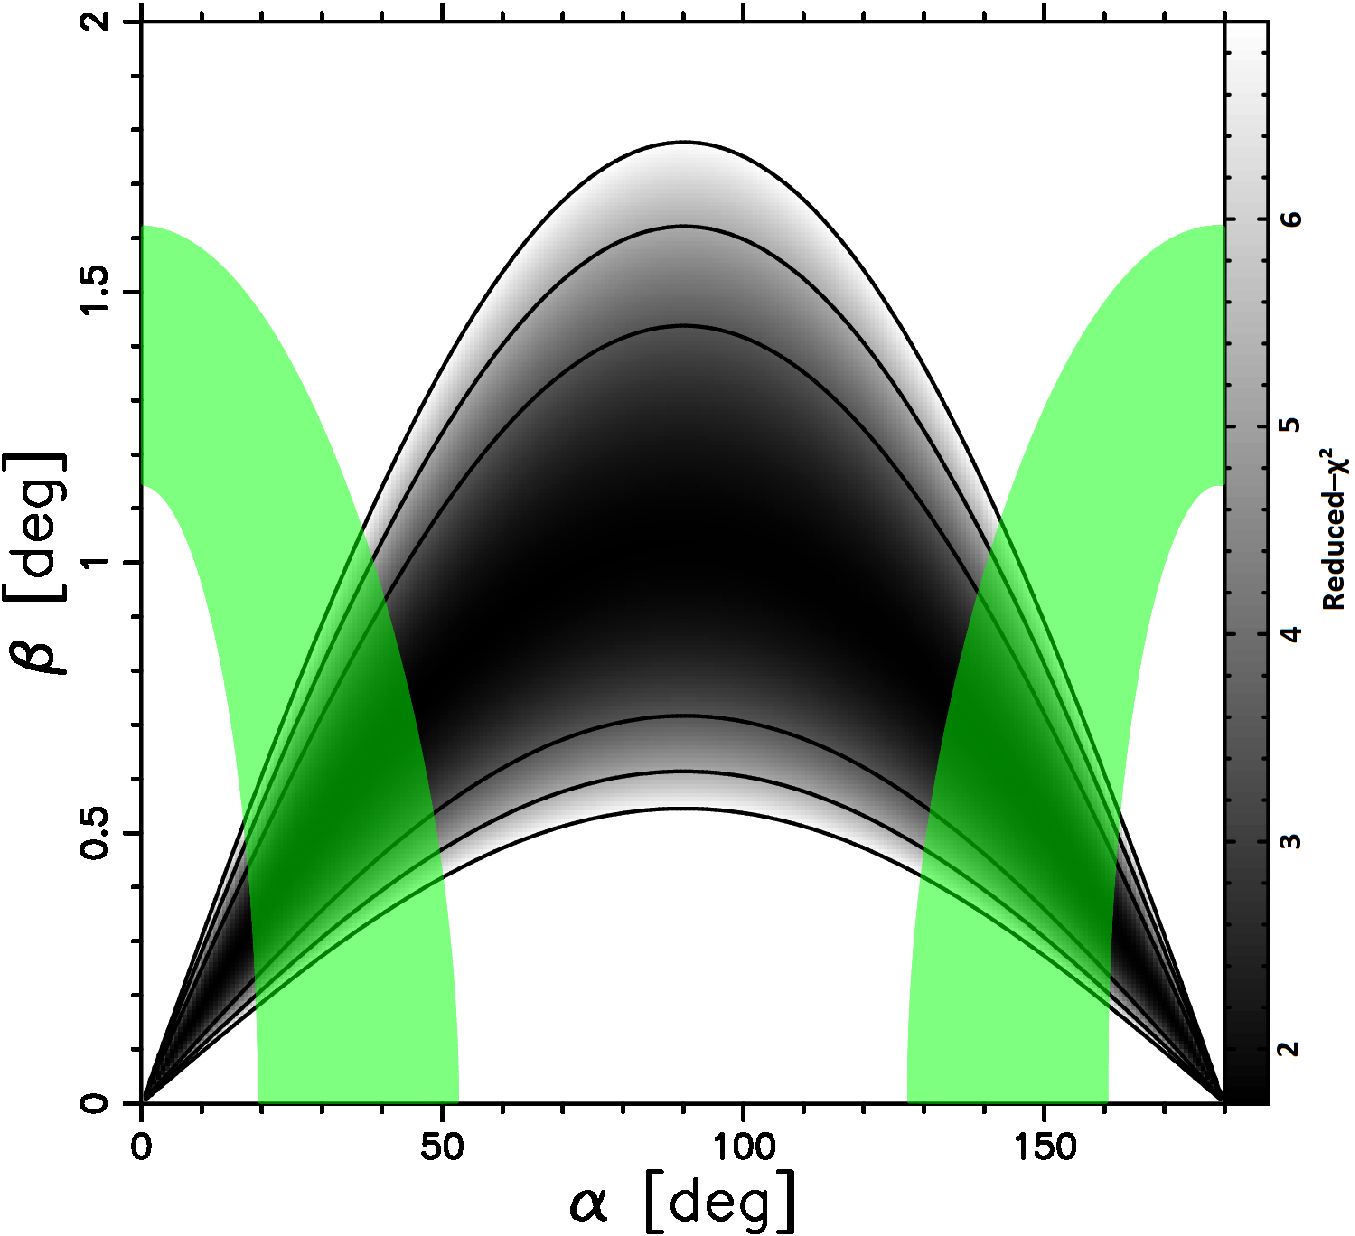
\includegraphics[width=0.6\textwidth]{Figures/J0250/banana.pdf}
        \caption[The goodness-of-fit of the RVM to the PSR~J0250+5854 PA curve]{The goodness-of-fit (reduced-$\chi^2$) of the RVM to the PA curve as a function of ($\alpha$, $\beta$) space obtained for the LOFAR Core data is shown in grey-scale. The black contours correspond to a reduced-$\chi^2$ of two-, three-, and four-times the minimum value. The green shaded regions are the `allowed' viewing geometries, which are constraints arising from the estimated emission height and observed profile width.}
        \label{fig: J0250 - banana}
    \end{center}
\end{figure}

Given the very small duty-cycle, limited information is available about how the PA varies with pulse longitude, and as a consequence $\alpha$ and $\beta$ are highly correlated when the RVM is fitted. The change of PA with pulse longitude is most rapid at the inflection point, $\sim$55~deg~deg$^{-1}$, which is predicted by the RVM to be equal to $\sin\alpha / \sin \beta$ \citep{Kxxx1970}. This implies that $\beta$ must be small ($\lesssim1.8\degr$) as expected for a detection of a slowly rotating pulsar with a narrow beam directed along the direction of the magnetic axis. The magnetic inclination angle $\alpha$ is unconstrained from RVM fitting alone.


The measured profile width provides additional information about the opening angle of the radio beam, how the line of sight cuts it, and the emission height. This can be used to further constrain $\alpha$ and $\beta$ in the same way as was done in Chapter~\ref{chapt: J1926} for PSR~J1926$-$0652 \citep[see also][]{RWJx2015a}. It is assumed that all radiation of a given frequency is produced at some height $h_\mathrm{em}$ in the magnetosphere in a circular region surrounding the magnetic axis. The emission beam is delimited by tangents to the last open field lines, forming a conal beam. At low emission altitudes, $h_\mathrm{em} \ll R_\mathrm{LC}$ (where $R_\mathrm{LC}$ is the light cylinder radius), the small angle limit applies, and the half opening angle of the emission cone is given by 
\begin{equation}
\label{eq: J0250 - cone angle}
    \rho \approx \sqrt{\frac{9\pi h_\mathrm{em}}{2cP_1}}.
\end{equation}
This relationship implies that the radio beam should widen with increasing emission height, and longer period pulsars can be expected to have narrower beams. The emission height at FAST frequencies (1250~MHz) is assumed to lie within the range of 200 to 400~km, which is the range expected for non-recycled pulsars at 1.4~GHz \citep[e.g.][]{MRxx2002, JKxx2019} -- this then corresponds to a half-opening angle of the beam $\rho \simeq 1 - 2\degr$ from Eq.~\eqref{eq: J0250 - cone angle}. 

The observed width of the pulse profile depends on how the line of sight cuts through the emission beam. \citet{GGRx1984} showed that the rotational phase range for which the line of sight samples the open-field-line region, $W$, can be expressed as
\begin{equation}
\label{eq: J0250 - allowed geometry}
    \cos\rho = \cos\alpha\cos(\alpha+\beta)+\sin\alpha\sin(\alpha+\beta)\cos\bigg(\frac{W}{2}\bigg).
\end{equation}
This means that a measurement of $W$ can help to constrain the parameters $\alpha$ and $\beta$, as well as $h_\mathrm{em}$ via $\rho$. Here it is important to note that the open-field-line region does not necessarily emit over its full extent, and hence the measured profile width may not necessarily correspond to $W$ as defined in Eq.~\eqref{eq: J0250 - allowed geometry}.

For the FAST profile $W_{10}=4.3\pm0.2\degr$, the width of the profile as defined at 10~per~cent of the peak flux density. This is believed is likely to correspond to a more fully illuminated beam than the LOFAR Core profile (see Sec.~\ref{sec: J0250 - discussion - profile width}). Moreover, $W$ as defined in Eq.~\eqref{eq: J0250 - allowed geometry} is assumed to be between the measured $W_{10}$ and twice the distance between the PA curve inflection point and the furthest edge of the FAST pulse profile, in order to account for potential underfilling of the radio beam (see Sec.~\ref{sec: J0250 - discussion - geometry} for the motivation). Here the PA inflection point is taken to coincide with the total intensity fiducial plane position, because the emission height at FAST frequencies is argued to be low enough to make any A/R effects small (see Sec.~\ref{sec: J0250 - discussion - geometry}). Taking into account the uncertainties on $W_{10}$ and the inflection point, this results in $4.1\degr \leq W \leq 6.9\degr$ assuming that at least one edge of the profile corresponds to the boundary with the last-open-field-line region.

This allowed range of $W$ and emission height results in a collection of contours in ($\alpha$, $\beta$) space defined by Eqs.~\eqref{eq: J0250 - cone angle}~and~\eqref{eq: J0250 - allowed geometry}. These contours (green shaded regions Fig.~\ref{fig: J0250 - banana}) show that $\beta$ is likely $\leq1.1\degr$, and suggests that the pulsar is relatively aligned: $20 \lesssim \alpha \lesssim 50\degr$, or $130 \lesssim \alpha \lesssim 170\degr$ for the opposite pole. Further to these considerations, it cannot be ruled out that neither edge of the FAST profile reaches the edge of the open-field-line region. This would correspond to a lower filling fraction and allow the magnetic and rotation axes to be modestly more aligned compared to what has been derived here. 

Given the emission height is unlikely to be higher at FAST frequencies, the narrower LOFAR Core profile at a lower frequency is therefore indicative of a smaller fraction of the open-field-line region being active. This is discussed further in Sec.~\ref{sec: J0250 - discussion}.
























\subsection{Flux density spectrum}
\label{sec: J0250 - analysis - flux}

With a factor of $\sim$5 increase in spectral coverage with respect to \citet{TBC+2018}, the radio spectrum of PSR~J0250+5854 could be further quantified. Flux calibration of the FAST data was possible by utilising the observation of the nearby BL Lacertae object J0303+472, which was used as a reference source (see Sec.~\ref{sec: J0250 - observations}). This source, also known by the identifier 4C~47.08 \citep{VVxx2006}, has a known flux density of 1.8~Jy at a wavelength of 20~cm (approximately 1500~MHz, suitably close to the centre frequency of the FAST data at 1250~MHz) as listed in the VLA Calibrator List\footnote{\url{https://science.nrao.edu/facilities/vla/observing/callist}}. The NASA/IPAC Extragalactic Database (NED)\footnote{\url{https://ned.ipac.caltech.edu/}} entry for this object contains a list of flux densities of this source at different frequencies from the literature, revealing a significant scatter in flux density measurements of observations at similar frequencies. To accommodate this scatter, as well as the uncertainty in the intrinsic flux because of interstellar scintillation, an uncertainty of 50~per~cent was assigned to the flux density. This is consistent practice with other work on pulsar flux density measurements \citep[e.g.][]{Sxxx1973}. The flux density calibration was performed using the \textsc{pac} routine in \textsc{psrchive}, and a flux density of $4\pm2$~$\upmu$Jy was measured for PSR~J0250+5854 at 1250~MHz. The S/N of the profile is also consistent with what is predicted for this flux density by the radiometer equation (see Sec.~\ref{sec: intro - observation processing - flux calibration}) with known (zenith angle-dependent) values for the gain $G = 14$~K~Jy$^{-1}$ and system temperature $T_\mathrm{sys} = 25$~K of FAST\footnote{see also Appendix 2 of \url{http://english.nao.cas.cn/focus2015/201901/t20190130_205104.html}} \citep{LWQ+2018}. This flux density is below the upper limits at a similar frequency based on non-detections with the Lovell and Nan\c{c}ay telescopes \citep[0.009~mJy and 0.015~mJy resepectively, ][]{TBC+2018}.

Figure~\ref{fig: J0250 - spectrum} shows the flux density of PSR~J0250+5854 as a function of observing frequency, and includes the flux densities previously measured by \citet{TBC+2018}. These previous measurements include detections with the GBT, the LOFAR HBAs, and a flux density measurement obtained from the LOFAR Two-meter Sky Survey \citep[LoTSS;][]{SRB+2017}.
\begin{figure}
    \begin{center}
        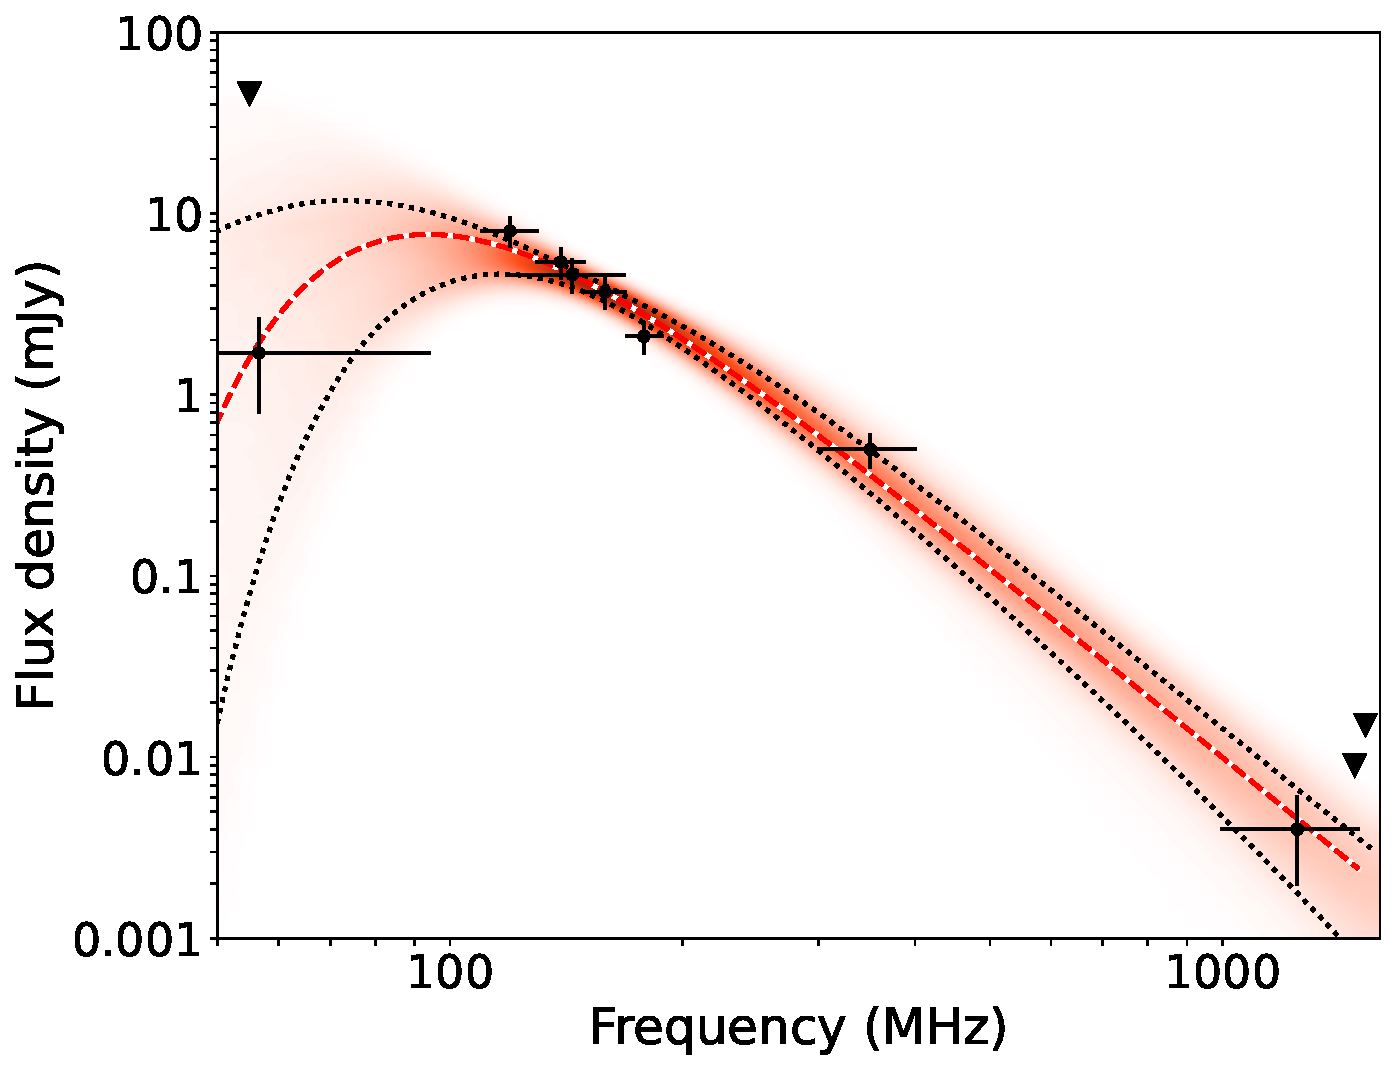
\includegraphics[width=0.6\textwidth]{Figures/J0250/spectral_index_turnover.pdf}
        \caption[The radio frequency flux density spectrum of PSR~J0250+5854]{The flux density spectrum of PSR~J0250+5854, including upper limits (inverted triangles) from previous non-detections \citep{TBC+2018}. As in Fig.~\ref{fig: J0250 - width evolution}, the horizontal error bars indicate the bandwidth of a given observation. This plot includes the previous flux density measurements from Tan et al., with the new addition of the NenuFAR and FAST measurements. A power-law relationship with a low-frequency turnover was fitted to the data, and the best fit is indicated by the red and white dashed line. The distribution of acceptable fits is shown, similar to Fig.~\ref{fig: J0250 - width evolution}. The NenuFAR bandwidth extends down to 19~MHz, beyond what is shown in the figure. The fitted parameters from Eq.~\eqref{eq: J0250 - spectrum} are the scaling factor $b = 0.1^{+0.3}_{-0.0}$, turnover parameter $m = 2.1^{+0.0}_{-1.2}$, critical frequency $\nu_c = 94\pm24$~MHz, and spectral index $k = -3.5^{+0.2}_{-1.4}$.}
        \label{fig: J0250 - spectrum}
    \end{center}
\end{figure}
The detection of PSR~J0250+5854 at 57~MHz using NenuFAR marks the lowest frequency detection that is published. The flux density of the pulsar at this frequency was estimated using the radiometer equation (Eq.~\eqref{eq: intro - pulsar radiometer equation}), and was found to be $1.7\pm0.9$~mJy, where a 50~per~cent uncertainty is again assigned. In calibrating these data the elevation of the source and number of antennas in the array were taken into account as these parameters affect the gain, as does the bandpass of the array. The sky background temperature was estimated to be 9050~K at the position of PSR~J0250+5854 (which dominates over the receiver temperature of 776~K), found by extrapolating the sky temperature measured at 408~MHz \citep{HSSW1982} with a spectral index of $-2.55$ \citep{LMOP1987, RRxx1988} to the centre frequency of 56.54~MHz. Full details of the NenuFAR flux calibration procedure are to be published in the instrumentation paper (Zarka et al., in prep.). This measurement shows that the spectrum of PSR~J0250+5854 rolls over at low frequencies, and this explains the lack of a detection at a similar frequency reported by \citet{TBC+2018} based on LOFAR Low Band Antenna array observations (the upper limit for these was calculated to be $<46$~mJy). The spectral shape of PSR~J0250+5854 is further discussed in Sec.~\eqref{sec: J0250 - discussion - flux density}.








\section{Discussion}
\label{sec: J0250 - discussion}

\subsection{Flux density and spectral index}
\label{sec: J0250 - discussion - flux density}

The emission of PSR~J0250+5854 is weak at a centre frequency of 57~MHz as observed with the NenuFAR telescope (compared to its flux density at 150~MHz), which is the result of a spectral turnover (see Sec.~\ref{sec: J0250 - analysis - flux}). This is not unusual in the pulsar population: for example, \citet{BKK+2016} noted that 25~per~cent of their low-frequency sample were fitted by a broken power law with a turnover typically around 100~MHz. Furthermore, \citet{JSK+2018} noted that 21~per~cent of their sample deviates from a simple power law, exhibiting mainly broken power laws or low-frequency turnovers. The physical reasons for this are uncertain, but their analysis suggests that the deviations are partially intrinsic to the pulsar emission or because of magnetospheric absorption processes, and partially due to the environment around the pulsar or effects of the ISM.

To quantify the spectral turnover of PSR~J0250+5854, a power law with a low-frequency turnover was fitted to the data using the same model used by \citet{JSK+2018}. This takes the form
\begin{equation}
\label{eq: J0250 - spectrum}
    S_\nu = b \bigg(\frac{\nu}{\nu_0}\bigg)^k \exp\bigg( \frac{k}{m} \bigg(\frac{\nu}{\nu_c}\bigg)^{-m}\bigg),
\end{equation}
where $\nu_0 = 500$~MHz is a constant (and arbitrary) reference frequency. The fitted parameters are $b$, a constant scaling factor; $k$, the spectral index; $\nu_c$, the turnover frequency; and $m$ which determines the smoothness of the transition. The value of $m$ is expected to be positive, and $\leq2.1$.

With only one flux density measurement below the turnover frequency, the parameters are somewhat ill-defined. The optimal fit\footnote{The resulting probability density function of $m$ is highly clustered at the maximum allowed value of $2.1$ which was implemented as a prior. Therefore, no meaningful uncertainty on $m$ could be assigned.} (Fig.~\ref{fig: J0250 - spectrum}, red and white dashed line) is for an exponent $m=2.1$. This corresponds to the sharpest turnover allowed within the free-free absorption model (see \citet{JSK+2018} and references therein). The fitted spectral index of $k = -3.5^{+0.2}_{-1.4}$ is steep compared to the mean found for the pulsar population, but not excessively so: \citet{BLVx2013} found a mean spectral index of $-1.4$ with unit standard deviation, whilst \citet{JSK+2018} found a mean of $-1.60$ with a standard deviation of 0.54. Other examples of such steep spectral indices exist, including PSR~J1234$-$6423 which has a broken power-law spectrum with a spectral index of $-3.8\pm0.5$ below $\sim$1700~MHz \citep{JSK+2018}.

\citet{TBC+2018} noted that there are occasional bright pulses at 350~MHz (GBT data) in the leading component of the profile of PSR~J0250+5854. This behaviour was not seen in the LOFAR observations at around 150~MHz. If equally bright single pulses exist in the FAST frequency band, then they should be comfortably detectable above the level of the thermal noise. However, the residual baseline variations in the single pulse data are such that these bright pulses cannot be confidently detected. It therefore remains to be seen how the erratic nature of the single pulses evolves above frequencies of 350~MHz.











\subsection{Profile width evolution}
\label{sec: J0250 - discussion - profile width} 
As can be seen in Fig.~\ref{fig: J0250 - width evolution}, the profile width of PSR~J0250+5854 increases with observing frequency, from around $1\degr$ at 150~MHz to $2\degr$ at 1250~MHz. Equation~\eqref{eq: J0250 - thorsett relation} was fitted to the measured profile widths as a function of frequency, resulting in a power-law index $B = 1.9\pm0.4$ (see Sec.~\ref{sec: J0250 - analysis - profile widths}). Although it is unusual for pulsars to have a positive index, meaning that their profiles broaden with increasing frequency, a number of other examples are known. \citet{CWxx2014} identified 29 pulsars out of 150 with such a positive index based on profiles from the EPN database. Given the relatively large uncertainty on both this measured value of $B$ and those measured by \citet{CWxx2014}, the index for PSR~J0250+5854 is consistent with 24 out of the 29 pulsars with a reported positive index. None of these 29 pulsars have a significantly larger $B$ than that of PSR~J0250+5854. This increase in profile width with frequency is contrary to the expectation from RFM, and possible reasons are discussed here and in Sec.~\ref{sec: J0250 - discussion - geometry}.

Higher frequency radiation can be expected to be produced closer to the neutron star. This follows from models based on curvature radiation from relativistic bunches of particles travelling along the magnetic field lines \citep[e.g.][and references therein]{GLMx2004,DRxx2015}, as well as those based on plasma instabilities since both the plasma density and the plasma frequency decrease with increasing altitude (e.g. \citealt{HAxx2001} and references therein; also \citealt{GGMx2002}). As a consequence, the opening angle of the radio beam can be expected to be narrower at higher frequencies, unless a larger fraction of the open-field-line region becomes active. \citet{PHS+2016} studied 100 pulsars and measured their profile widths at frequencies ranging from tens of megahertz up to 1400~MHz. Only in a few cases (for example PSRs~B1541+09, B1821+05, B1822$-$09, and B2224+65) was the profile width seen to increase significantly with frequency. In these examples, profile broadening was indeed caused by the emergence of new profile components as frequency increased pointing to more field lines becoming active.

% A clear example of profile evolution with frequency due to multiple components is seen in PSR~B1919+21 as studied between 48 and 1700~MHz by \citet{HSH+2012}. The profile of this pulsar consists of two components which appear to move apart as frequencies increases. As this happens, one component becomes narrower, whilst the other broadens. Similarly, PSR~B0809+74 has a profile which was also modelled with two Gaussian components \citep{HSH+2012}. As frequency increases from 15 to 7850~MHz, the trailing component drifts to earlier phases, passing the fiducial component to end up on the leading side of the profile. Both these examples are difficult to explain by RFM alone.

Observations at a frequency around 800~MHz could help reveal the reasons for the abnormal frequency evolution of the profile of PSR~J0250+5854. The profile morphology is indeed complex, with a skewed profile shape in both the LOFAR Core and FAST observations. The GBT profile shows a distinct double-peaked structure, with distinct behaviours: \citet{TBC+2018} noted that the stronger first component was caused by occasional strong individual pulses. At other frequencies no well separated profile components are observed. However, the flattened peak in the LOFAR Core profile is suggestive of two blended components of similar intensity. This flattening was not visible for the profiles published in \citet{TBC+2018}, which is because of the lower S/N. By inspecting all available data, no significant profile shape variability has been detected in LOFAR Core observations of PSR~J0250+5854.
















\subsection{Emission height and viewing geometry}
\label{sec: J0250 - discussion - geometry}

Constraining the viewing geometry is particularly interesting for slowly rotating pulsars, as it can highlight differences with magnetars (see Sec.~\ref{sec: J0250 - discussion - magnetar comparison}). As seen in Fig.~\ref{fig: J0250 - polarised profiles}, the inflection point of the PA swing occurs very close to the centre of the FAST profile, and is within the observable pulse at LOFAR frequencies. This implies that the emission height at both frequencies must be considerably smaller than the light cylinder radius, which itself is large ($1.123\times10^{6}$~km) due to the star's slow rotation. If the emission heights were not low, relativistic aberration and retardation (A/R) effects would shift the inflection point outside the span of the pulse profile. \citet{BCWx1991} showed that the expected delay in pulse longitude between the inflection point and the longitude in the profile corresponding to the fiducial plane (the plane containing the magnetic and rotation axes) is $\Delta\phi = 4 h_\mathrm{em} / R_\mathrm{LC}$.

The lack of a significant A/R shift for either frequency affirms that radio pulsars produce emission at an absolute emission altitude, rather than being at a constant fraction of $R_\mathrm{LC}$. Given the emission height is not at a constant fraction of $R_\mathrm{LC}$ there should be a period dependence of the pulse width \citep[e.g.][]{Rxxx1993}. Based on this relationship \citet{KJxx2007} proposed that the maximum emission height of radio pulsars at 1.4~GHz is around 1000~km, refined to an absolute height range of 200 to 400~km irrespective of pulse period \citep{JKxx2019, JSKx2020}. This is the range assumed for the FAST profile at 1250~MHz.

There is a significant difference in the longitude of the inflection point of the PA curve between the LOFAR and FAST frequencies. This was found by fitting a RVM curve with the same $\alpha$ and $\beta$ to the FAST and LOFAR PA curves independently. The uncertainty on the locations of the inflection point ($\phi_0$) for each dataset was found using bootstrapping. The PA points were allowed to vary within their uncertainties (which were scaled to make the best fit have a reduced-$\chi^2$ of 1), and the PA offset and $\phi_0$ were optimised. This was repeated 1000 times, and the standard deviation of the distribution of $\phi_0$ was taken as the uncertainty on the best fit for each dataset. The offset between the inflection points was found to be $\Delta \phi_0 = 1.2\pm 0.2\degr$.

If this is interpreted as purely due to a difference in emission height between the FAST and LOFAR Core profiles, then the emission height at LOFAR frequencies would be about 6000~km higher than at FAST frequencies. This is on the large side -- for example, extending the empirical model of RFM for non-recycled pulsars by \citet{KGxx2003} to PSR~J0250+5854 suggests emission heights from $(1.2\pm0.3)\times 10^3$~km at FAST frequencies to $(3\pm1)\times10^3$~km at the much lower NenuFAR frequencies. So other effects may affect the measured $\Delta\phi_0$. It should be noted that alignment of the profiles depends on the DM assumed -- a change in the DM of $\sim$0.4~cm$^{-3}$~pc would produce the same results, although such a large difference is inconsistent with the frequency-resolved LOFAR Core data. 

Nevertheless, the evidence suggests that the LOFAR Core emission is produced at greater heights than the FAST profile, where the emission cone is wider. This makes the narrowness of the lower-frequency profiles even more striking, and emphasises that fewer open field lines are active at lower frequencies.















\subsection{Beam shape evolution and polar cap configuration}
\label{sec: J0250 - discussion - beam shape}

The narrowness of the LOFAR Core profile of PSR~J0250+5854 suggests that, at least at those frequencies, the beam is underfilled compared to the open-field-line region. In the framework of the core-cone model \citep[e.g.][]{Rxxx1983a,Rxxx1983b, RRxx1990, Rxxx1993} this can be explained by so-called conal outriders. Here, the more narrow central core component dominates at low frequencies. However, as the core emission has a steeper spectrum than the wider conal components, the latter can become more prominent at higher frequencies. Therefore, the broader FAST profile could be due to the rise in relative intensity of the conal components, giving the appearance of a broader beam if blended with the core component. 

This picture is also broadly consistent with the geometry obtained from the polarisation data. In this scenario, the LOFAR Core profile is associated with core beam emission, while the FAST profile is broader due to the presence of emission from the inner cone. The core beam does not change significantly with emission height, and is believed to reflect the size of the polar cap at the pulsar's surface \citep{Rxxx1983a}. \citet{Rxxx1990} found that the core beam width follows an empirical relation dependent on $\alpha$,
\begin{equation}
    \label{eq: J0250 - core beam W50}
    W_{50} =\frac{2.45\degr P_1^{-0.5}}{\sin\alpha}.
\end{equation}
The 23.5~s period of PSR~J0250+5854 and the measured width of the LOFAR Core profile $W_{50} \approx 1\degr$ would then give $\alpha \approx 30\degr$. The gradient of the PA curve at the inflection point $\sin\alpha/\sin\beta \approx 55$~deg~deg$^{-1}$, which then means $\beta \approx 0.5\degr$. These values of $\alpha$ and $\beta$ lie within the `allowed geometries' in Fig.~\ref{fig: J0250 - banana}, which were derived without a specific beam model in mind. Going further, \citet{Rxxx1993} argues that the half opening angle of the inner cone follows the relation
\begin{equation}
    \label{eq: J0250 - inner cone rho}
    \rho_\mathrm{inner} = 4.3\degr P_1^{-0.52},
\end{equation}
which for this pulsar gives $\rho_\mathrm{inner} = 0.83\degr$. Substituting these derived values for $\alpha$, $\beta$, and $\rho_\mathrm{inner}$ into Eq.~\eqref{eq: J0250 - allowed geometry} gives the expected width of the inner cone of $W \approx 2.5\degr$. This is consistent with $W_{50} = 2.4\pm 0.1\degr$ measured for the FAST profile, and so reinforces the conal outrider hypothesis. It is expected that the profile would evolve into a wide, double-peaked profile at even higher radio frequencies. The bifurcated GBT profile in Fig.~\ref{fig: J0250 - profiles} would therefore correspond not to conal emission, but should instead be associated with a magnetospheric absorption feature of a core-single profile, which are known to occur between 200 to 800~MHz \citep[e.g.][]{Rxxx1983b, Rxxx1986}. 

As pointed out in Sec.~\ref{sec: J0250 - discussion - profile width}, the doubling of the profile width over the frequency range covered is unusual in the population, and there are no clear signs of the emergence of extra profile components. The physical reasons for the profile widening could therefore differ from the core-cone model explanation, and alternative models should also be explored.

As highlighted in the introduction, the slow rotation of PSR~J0250+5854 implies a tiny polar cap connected to the open-field-line region. One can wonder if there is enough space to fully develop the type of beam complexity encountered in more typical pulsars. In the model of \citet{MBMA2020} it is predicted that the polar cap of PSR~J2144$-$3933 is only large enough to support a single pair-production site -- known as a `spark' -- hence its profile would be a single component. For PSR~J0250+5854 (which although slower has a much larger spin-down rate $\dot{P}$) their model predicts that the footprint of a spark is one fifth of the area of the polar cap, meaning that up to three sparks could be supported if they are packed tightly. Moreover, sparks are also required to be separated from one another due to screening effects, and this separation is believed to be of the order of the spark size itself \citep[e.g.][]{GSxx2000} meaning that the polar cap may only be able to support a single spark. In the framework of cores and cones it may explain why the profile appears core dominated whilst lying in a part of the $P$-$\dot{P}$ diagram inhabited by older, less energetic pulsars. These are thought to be cone-dominated due to their lower rate of energy loss as argued by \citet[based on the plasma generation model of \citealt{THxx2015}]{ROWx2020}. But it could suggest that the profile widening at higher frequencies is not because of the emergence of conal emission.

\citet{CWxx2014} conclude that in a number of cases the widening of the profile at higher frequencies could not be ascribed to structures consistent with the core-cone model. This also appears to be the case in a small sub-group of pulsars studied by \citet{PHS+2016}. Like PSR~J0250+5854, these pulsars do not show well-separated profile peaks at the highest frequencies. The expectation from conventional RFM is based on emission being produced over a wide range of altitudes, and each height producing a distinct frequency. On the other hand, if a narrow range of emission heights generates broadband emission the observed spectrum will be different. This led \citet{CWxx2014} to suggest that fan beams could accommodate anti-RFM-like behaviour. Broadband emission is incorporated into the fan beam model \citep{Mxxx1987, DRDx2010, DRxx2012, DRxx2013, WPZ+2014} where emission is produced along magnetic flux tubes that extend out from the pole in a fan-like structure. A single fan, hence spark, would be required to explain the beam structure of PSR~J0250+5854. Support for this beam structure is found in observations of the precessing pulsars J1141$-$6545 and J1906+0746 \citep{MKS+2010, DKC+2013}. Following the suggestion of \citet{Mxxx1987} that each flux tube may have its own spectrum, \citet{CWC+2007} argued that the emission spectrum may not be homogeneous across a flux tube. In particular, they argue that pulsars which show pulse broadening with increasing frequency may have a flattening emission spectrum away from the magnetic axis, as supported by their simulations. Broadband emission in flux tubes with a location-varying spectral index follows naturally from particle-in-cell simulations of vacuum-gap pair-production \citep{Txxx2010} which predict that the momentum spectrum of the secondary plasma is not necessarily monotonic as a function of height within the magnetosphere, and so a given observed frequency cannot be assigned to a unique altitude.


















\subsection{Comparison to other slow pulsars and magnetars}
\label{sec: J0250 - discussion - magnetar comparison}

The extremely long period of PSR~J0250+5854 places it on the far right-hand side of the $P$-$\dot{P}$ diagram, in an area largely inhabited by magnetars and XDINSs. Since it is believed that the pulse period is a key factor controlling the width of radio pulse profiles, it is worth comparing PSR~J0250+5854 with the radio-emitting magnetars and other slowly spinning rotation-powered radio pulsars. This comparison can highlight what other parameters play a role in the radio beam geometry of these slowly rotating objects.  Despite the fact that magnetars form a distinct class of objects with much greater spin-down rates, and hence much higher rates of loss of rotational energy $\dot{E}$, they may evolve with time towards the parameter space occupied by the slow pulsars \citep[e.g.][]{VRP+2013}. However, the non-detection of PSR~J0250+5854 in X-rays makes such a connection uncertain \citep{TBC+2018}. Moreover, PSR~J0250+5854 is located squarely in the Galactic plane (at Galactic coordinates $l=137.7\degr$, $b=-0.5\degr$) which argues that it is still relatively young.

Aside from PSR~J0250+5854, the two other slowest-spinning known radio pulsars are PSRs~J2251$-$3711 ($P_1=12.1$~s), and J2144$-$3933 ($P_1=8.5$~s). There are five known magnetars for which pulsed radio emission has been detected: 1E~1547.0$-$5408 \citep{CRHR2007a}, PSR~J1622$-$4950 \citep{LBB+2010}, PSR~J1745$-$2900 \citep{EFK+2013}, XTE~J1810$-$197 \citep{CRH+2006}, and Swift~J1818.0$-$1607 \citep{ERB+2020, LSJB2020}. A summary of their properties is shown in Table~\ref{tab: J0250 - magnetar comparison}.
\begin{table}
	\centering
	\caption[Properties of the slow rotation-powered pulsars and radio magnetars]{Parameters (period $P_1$, spin-down rate $\dot{P}$) of the three slowest-spinning radio pulsars (top three sources) and the five magnetars (lower five sources) known to produce pulsed radio emission. The profile width of the radio pulsars are measured values of $W_{50}$ taken from this work and the referenced literature. The widths of the magnetar profiles are estimated based on the full extent over which significant emission was visible in the published profiles (at the reference frequency) in order to capture the complexity of the magnetar profiles. \newline \textbf{References:} (1) \citet{YMJx1999}; (2) \citet{MBMA2020}; (3) \citet{MKE+2020}; (4) \citet{CRHR2007a}; (5) \citet{CRJ+2008}; (6) \citet{LBB+2010}; (7) \citet{LBB+2012}; (8) \citet{EFK+2013}; (9) \citet{CRH+2006}; (10) \citet{CRJ+2007b}; (11) \citet{KSJ+2007}; (12) \citet{LLD+2019}; (13) \citet{ERB+2020}; (14) \citet{LSJB2020}; (15) \citet{CCC+2020}.}
	\label{tab: J0250 - magnetar comparison}
	\begin{tabular}{lrrrrr} % 6 columns, alignment for each
		\hline
	    Object & $P_1$  & $\dot{P}$   & Profile Width & Ref. Freq.  & References\\
	           &  (s) & (s s$^{-1}$) & ($\degr$)     &       (MHz) &           \\        
		\hline
		PSR~J0250+5854          & 23.5 & $2.72\times10^{-14}$ &  $2.0$ & 1250 & This work\\
		PSR~J2144$-$3933        & 8.5  & $4.96\times10^{-16}$ &  $0.8$ & 1400 & 1, 2\\
		PSR~J2251$-$3711        & 12.1 & $1.31\times10^{-14}$ & $1.2$  & 1382 & 3\\
		\hline
		1E~1547.0$-$5408        & 2.1  & $2.32\times10^{-11}$ & $90$   & 6600 & 4, 5\\
        PSR~J1622$-$4950        & 4.3  & $1.70\times10^{-11}$ & $190$  & 1400 & 6, 7\\
        PSR~J1745$-$2900        & 3.8  & $6.80\times10^{-12}$ & $15$   & 2400 & 8\\
        XTE~J1810$-$197          & 5.5  & $1.02\times10^{-11}$ & $35$   & 1400 & 9, 10, 11, 12\\
        Swift~J1818.0$-$1607    & 1.4  & $9\times10^{-11}$    & $20$   & 1548 & 13, 14, 15\\
		\hline
	\end{tabular}
\end{table}

Although the focus here is the differences in profile widths, it should be noted that there are other differences between the two classes of object, such as the spectra of magnetars being radically different and their radio emission being much more transient with periods of activity and strongly changing profile shapes, as studied by \citet{SSW+2009, DJW+2018, LLD+2019, DLB+2019,LJS+2021}.
Compared to the slow pulsars, the magnetars can have exceptionally shallow radio spectra. PSR~J1622$-$4950 has a flat spectrum between 1.4 and 24~GHz \citep{KJLB2011} similar to the spectra of 1547.0$-$5408 and XTE~J1810$-$197 \citep{CRJ+2007b, CRHR2007a, KSJ+2007}. In contrast, the spectral index of the slow pulsar PSR~J0250+5854 is exceptionally steep ($-3.5^{+0.2}_{-1.4}$ compared to the mean of $-1.6$ for the non-recycled pulsar population \citealt{JSK+2018}). However, the spectral index of the magnetar Swift J1818.0$-$1607 is relatively steep as well at $-2.26^{+0.02}_{-0.03}$ \citep{LSJB2020}, which led them to believe there may be a link with the rotationally powered PSR~J1119$-$6127 \citep[e.g][]{MPD+2017,DJW+2018}. Recently, \citet{CCC+2020} have shown that the spectral index of this object varies with time. 

The three slowest-spinning radio pulsars have long periods and narrow, fairly simple pulse profiles. Measurements of $W_{50}$ are published for these profiles and are representative of the overall profile width. Despite being the slowest-spinning of the three, PSR~J0250+5854 has the widest profile by around a factor of two. If only the period determines the width, the inverse would be expected. This suggests that besides PSR~J0250+5854 (see Sec.~\ref{sec: J0250 - discussion - geometry}) underfilling of the beam also plays a role in the other slow pulsars. In contrast, the magnetars have fairly complex profiles with multiple components of differing intensity, which means that $W_{50}$ is not always a representative number for the overall width of the profile. Therefore, for the magnetars the profile width as quoted in Table~\ref{tab: J0250 - magnetar comparison} spans the region where the emission in the published profiles is clearly distinguishable from the noise (rounded to the nearest five degrees).

Looking at Table~\ref{tab: J0250 - magnetar comparison} it is clear there is a stark contrast between the profile widths of the magnetars compared to the slow pulsars, much more than can be expected from just the differences in $P$ (and hence $R_\mathrm{LC}$). There are four potential geometric explanations for why magnetars have much wider profiles compared to the slow pulsars: 1) the three slowly rotating pulsars are observed with an extremely grazing line of sight with respect to the radio beam; 2) for the slowly rotating pulsars only a tiny fraction of the open-field-line region is active; 3) all magnetars have a magnetic axis almost aligned with the rotation axis; 4) all magnetars have atypically wide beams due to large emission heights or otherwise. In the following, I argue that only options 3) and 4) are viable, and that option 4) plays a more significant role. Option 1) relies on a very unlikely coincidence, and will not be considered further. 

It was argued in Sec.~\ref{sec: J0250 - discussion - profile width} that only part of the open-field-line region is active for PSR~J0250+5854. However, this fraction needs to be very small for this and the other slow pulsars if it is to be the main reason why the slow pulsars have such narrow beams compared to the magnetars. This seems unlikely to be the case, as it would not explain why there are no slow pulsars with multiple narrow profile components spread over a similar fraction of the rotation period for which magnetars show emission. Instead, the structure of the profiles of the slow pulsars blend together in a single narrow profile, whereas the magnetar profiles have much more complex, multi-component structure. The magnetars often exhibit individual components which are much wider than the full profiles of the slow pulsars.




% Paragraph(s) on magnetic alignment

If magnetars have very aligned radio beams with respect to their rotation axis (small $\alpha$), the observer's line of sight would spend a larger fraction of the time within the beam -- this can be seen by rearranging Eq.~\eqref{eq: J0250 - allowed geometry} for a fixed cone angle $\rho$ and impact parameter $\beta$. The process of Sec.~\ref{sec: J0250 - analysis - polarisation and geometry} can be used to estimate how extreme the alignment of the magnetars should be in order to explain their wide pulse profiles. Taking the mean magnetar period and median magnetar profile width from Tab.~\ref{tab: J0250 - magnetar comparison} with an emission height of 400~km (to be the same as the slow, non-recycled pulsars), such an object requires $\alpha\lesssim 11\degr$ to produce profiles of the observed width. If true, this would require that these young objects have beams which become aligned much faster compared to what is believed to happen for normal pulsars \citep{TMxx1998,WJxx2008} if they are born with a random $\alpha$ distribution.


However, there is little evidence to suggest that magnetars have a systematically smaller $\alpha$ compared to the slow pulsars. Alignment of the magnetic and rotation axes was suggested by \citet{CCR+2007} for XTE~J1810$-$197, although with orthogonal polarisation mode jumps it could be closer to orthogonality as well. \citet{KSJ+2007} preferred to interpret the polarisation of this magnetar with a non-aligned, offset dipole or a non-dipolar magnetic field configuration. An aligned magnetic field was suggested for 1E~1547.0$-$5408 \citep{CRJ+2008}, but RVM fitting for PSR~J1622$-$4950 by \citet{LBB+2012} suggested a configuration that is not particularly aligned. Furthermore, the slow pulsar PSR~J2144$-$3933 is thought to be a nearly orthogonal rotator \citep{MBMA2020}, as is the magnetar Swift~J1818.0$-$1607 \citep{LJS+2021}. An issue with attributing small $\alpha$ to magnetars is that it makes it difficult to reconcile with the large modulation of the thermal X-rays, as was highlighted for XTE~J1810$-$197 \citep{GHxx2007,PGxx2008} and 1E~1547.0$-$5408 \citep{IER+2010}.

Overall, the evidence from RVM fitting for magnetars having particularly small $\alpha$ values is mixed and X-ray data seem to preclude very small $\alpha$. Furthermore, if magnetars evolve into slowly spinning rotation-powered pulsars as they spin down, the latter objects should have small $\alpha$ values and correspondingly wide profiles as well. For PSR~J0250+5854, for example, the analysis shows that it is unlikely that $\alpha$ is very small. Therefore, it is concluded that the intrinsic emission cone properties must play a significant role in explaining the magnetar radio profile widths.



% Case 4) could the magnetars have intrinsically wider beams?

If the emission heights are the dominant reason for the magnetars having wider radio profiles, they need to be $\sim$20 times larger (around 10,000~km) compared to the slowly spinning rotation-powered pulsars. These large emission heights for the magnetars imply wide radio beams (Eq.~\ref{eq: J0250 - cone angle}). However, alternatively, if their radio beams are confined by last open field lines which close within the light cylinder (as suggested by detailed simulations by \citealt{Sxxx2006}; see also the discussion of `Y-points' by \citealt{Cxxx2014}), or if magnetic field sweepback plays a large role \citep[e.g.][]{CRxx2012} then their polar beams will be wider as well. Therefore, one cannot distinguish between large emission heights and extended open-field-line regions \citep[e.g.][]{RWJx2015b, RWJx2015a}. In such a scenario, the open-field-line regions of magnetars would need to be $\sim$5 times larger than predicted for a static dipole field. In either case, it would imply that slowly spinning rotation-powered pulsars have dramatically reduced beaming fractions compared to magnetars -- this could explain the deficit of observed slow pulsars near the death valley.

The large implied difference in the beaming fraction between the two classes of objects is unexpected given the weak $\dot{P}$ dependence of the pulse widths observed for the non-recycled pulsars \citep[e.g.][]{KGxx2003, JKxx2019}. This implies that for these slowly rotating objects the role of $\dot{P}$ in governing the beaming fraction is much larger than for the normal pulsar population. This could potentially be facilitated by the incredible strengths of the magnetar magnetic fields.

















\section{Conclusions}
\label{sec: J0250 - conclusions}

We have obtained the highest- and lowest-frequency radio detections of PSR~J0250+5854, the most slowly rotating radio-emitting pulsar known, using simultaneous observations from 57~MHz to 1250~MHz. While PSR~J0250+5854 is slow, its continued radio emission can be explained by, for example, the partially screened gap model. The highest frequency detection with FAST (1250~MHz) shows that the spectrum is exceptionally steep with a spectral index of $-3.5^{+0.2}_{-1.4}$ and the lowest frequency detection with NenuFAR (57~MHz) reveals a spectral turn-over below 95~MHz. The pulse profile shows a broadening at higher frequencies contrary to the expectations of radius-to-frequency mapping, which implies that the beam is underfilled at lower frequencies. The polarisation information of LOFAR Core data at 150~MHz and FAST data at 1250~MHz was used to constrain the viewing geometry. This shows that the line of sight impact parameter $\beta$ is very small, passing within $1.8\degr$ of the magnetic axis, and confirms that the radio beam is very narrow as expected for such a slow pulsar. Furthermore, the lack of a delay between the profile peak and position angle curve inflection point implies that the emission height of PSR~J0250+5854 at 1250~MHz is low, consistent with the 200 to 400~km range found for other non-recycled pulsars. Finally, comparisons are drawn between other slow pulsars, PSR~J0250+5854, and the five known magnetars with pulsed radio emission which have the most similar pulse periods in the known pulsar population. The profile widths of the magnetars are significantly broader than the normal slow pulsars -- it was argued that whilst magnetic alignment in magnetars may play a role in explaining this, the main reason is likely to be either considerably expanded open-field-line regions or substantially larger emission heights for magnetars.



